\documentclass[1p]{elsarticle_modified}
%\bibliographystyle{elsarticle-num}

%\usepackage[colorlinks]{hyperref}
%\usepackage{abbrmath_seonhwa} %\Abb, \Ascr, \Acal ,\Abf, \Afrak
\usepackage{amsfonts}
\usepackage{amssymb}
\usepackage{amsmath}
\usepackage{amsthm}
\usepackage{scalefnt}
\usepackage{amsbsy}
\usepackage{kotex}
\usepackage{caption}
\usepackage{subfig}
\usepackage{color}
\usepackage{graphicx}
\usepackage{xcolor} %% white, black, red, green, blue, cyan, magenta, yellow
\usepackage{float}
\usepackage{setspace}
\usepackage{hyperref}

\usepackage{tikz}
\usetikzlibrary{arrows}

\usepackage{multirow}
\usepackage{array} % fixed length table
\usepackage{hhline}

%%%%%%%%%%%%%%%%%%%%%
\makeatletter
\renewcommand*\env@matrix[1][\arraystretch]{%
	\edef\arraystretch{#1}%
	\hskip -\arraycolsep
	\let\@ifnextchar\new@ifnextchar
	\array{*\c@MaxMatrixCols c}}
\makeatother %https://tex.stackexchange.com/questions/14071/how-can-i-increase-the-line-spacing-in-a-matrix
%%%%%%%%%%%%%%%

\usepackage[normalem]{ulem}

\newcommand{\msout}[1]{\ifmmode\text{\sout{\ensuremath{#1}}}\else\sout{#1}\fi}
%SOURCE: \msout is \stkout macro in https://tex.stackexchange.com/questions/20609/strikeout-in-math-mode

\newcommand{\cancel}[1]{
	\ifmmode
	{\color{red}\msout{#1}}
	\else
	{\color{red}\sout{#1}}
	\fi
}

\newcommand{\add}[1]{
	{\color{blue}\uwave{#1}}
}

\newcommand{\replace}[2]{
	\ifmmode
	{\color{red}\msout{#1}}{\color{blue}\uwave{#2}}
	\else
	{\color{red}\sout{#1}}{\color{blue}\uwave{#2}}
	\fi
}

\newcommand{\Sol}{\mathcal{S}} %segment
\newcommand{\D}{D} %diagram
\newcommand{\A}{\mathcal{A}} %arc


%%%%%%%%%%%%%%%%%%%%%%%%%%%%%5 test

\def\sl{\operatorname{\textup{SL}}(2,\Cbb)}
\def\psl{\operatorname{\textup{PSL}}(2,\Cbb)}
\def\quan{\mkern 1mu \triangleright \mkern 1mu}

\theoremstyle{definition}
\newtheorem{thm}{Theorem}[section]
\newtheorem{prop}[thm]{Proposition}
\newtheorem{lem}[thm]{Lemma}
\newtheorem{ques}[thm]{Question}
\newtheorem{cor}[thm]{Corollary}
\newtheorem{defn}[thm]{Definition}
\newtheorem{exam}[thm]{Example}
\newtheorem{rmk}[thm]{Remark}
\newtheorem{alg}[thm]{Algorithm}

\newcommand{\I}{\sqrt{-1}}
\begin{document}

%\begin{frontmatter}
%
%\title{Boundary parabolic representations of knots up to 8 crossings}
%
%%% Group authors per affiliation:
%\author{Yunhi Cho} 
%\address{Department of Mathematics, University of Seoul, Seoul, Korea}
%\ead{yhcho@uos.ac.kr}
%
%
%\author{Seonhwa Kim} %\fnref{s_kim}}
%\address{Center for Geometry and Physics, Institute for Basic Science, Pohang, 37673, Korea}
%\ead{ryeona17@ibs.re.kr}
%
%\author{Hyuk Kim}
%\address{Department of Mathematical Sciences, Seoul National University, Seoul 08826, Korea}
%\ead{hyukkim@snu.ac.kr}
%
%\author{Seokbeom Yoon}
%\address{Department of Mathematical Sciences, Seoul National University, Seoul, 08826,  Korea}
%\ead{sbyoon15@snu.ac.kr}
%
%\begin{abstract}
%We find all boundary parabolic representation of knots up to 8 crossings.
%
%\end{abstract}
%\begin{keyword}
%    \MSC[2010] 57M25 
%\end{keyword}
%
%\end{frontmatter}

%\linenumbers
%\tableofcontents
%
\newcommand\colored[1]{\textcolor{white}{\rule[-0.35ex]{0.8em}{1.4ex}}\kern-0.8em\color{red} #1}%
%\newcommand\colored[1]{\textcolor{white}{ #1}\kern-2.17ex	\textcolor{white}{ #1}\kern-1.81ex	\textcolor{white}{ #1}\kern-2.15ex\color{red}#1	}

{\Large $\underline{11n_{179}~(K11n_{179})}$}

\setlength{\tabcolsep}{10pt}
\renewcommand{\arraystretch}{1.6}
\vspace{1cm}\begin{tabular}{m{100pt}>{\centering\arraybackslash}m{274pt}}
\multirow{5}{120pt}{
	\centering
	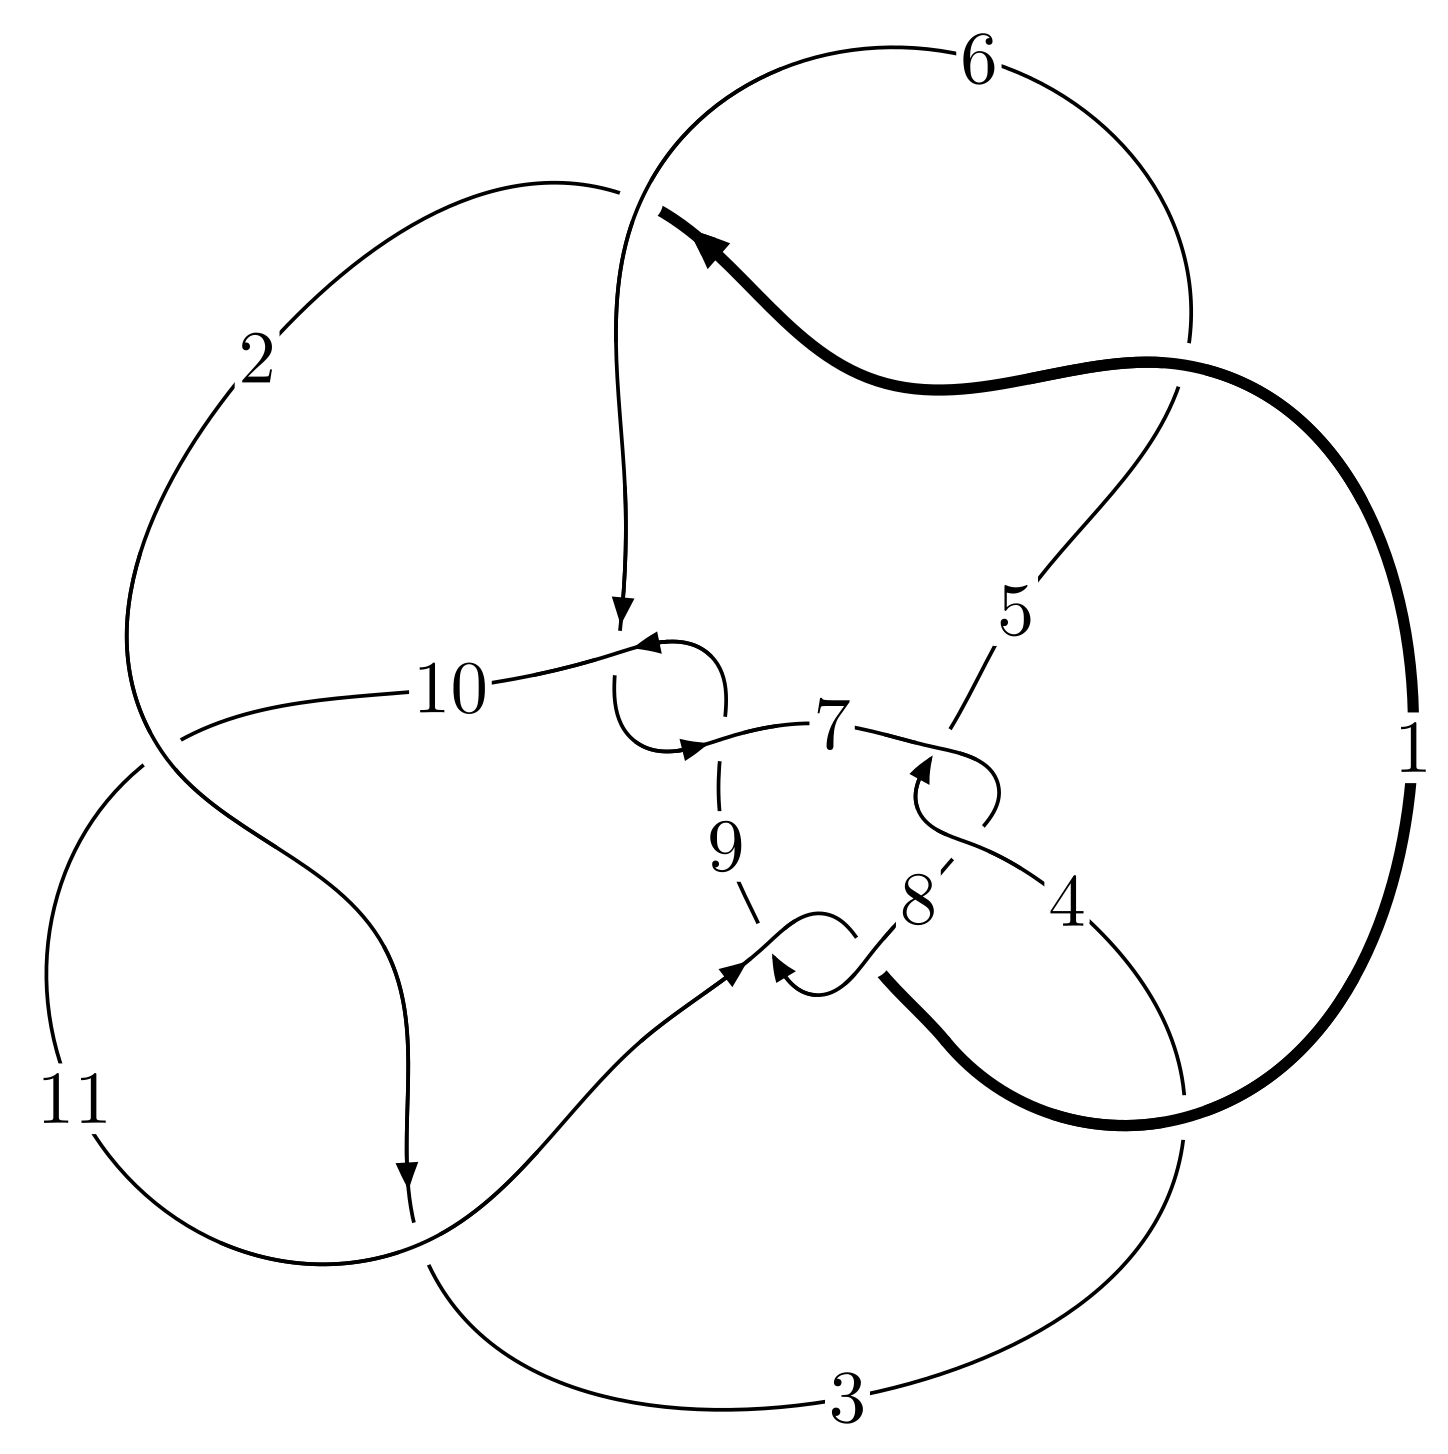
\includegraphics[width=112pt]{../../../GIT/diagram.site/Diagrams/png/795_11n_179.png}\\
\ \ \ A knot diagram\footnotemark}&
\allowdisplaybreaks
\textbf{Linearized knot diagam} \\
\cline{2-2}
 &
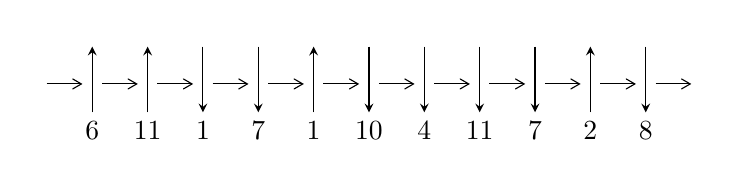
\begin{tikzpicture}[x=20pt, y=17pt]
	% nodes
	\node (C0) at (0, 0) {};
	\node (C1) at (1, 0) {};
	\node (C1U) at (1, +1) {};
	\node (C1D) at (1, -1) {6};

	\node (C2) at (2, 0) {};
	\node (C2U) at (2, +1) {};
	\node (C2D) at (2, -1) {11};

	\node (C3) at (3, 0) {};
	\node (C3U) at (3, +1) {};
	\node (C3D) at (3, -1) {1};

	\node (C4) at (4, 0) {};
	\node (C4U) at (4, +1) {};
	\node (C4D) at (4, -1) {7};

	\node (C5) at (5, 0) {};
	\node (C5U) at (5, +1) {};
	\node (C5D) at (5, -1) {1};

	\node (C6) at (6, 0) {};
	\node (C6U) at (6, +1) {};
	\node (C6D) at (6, -1) {10};

	\node (C7) at (7, 0) {};
	\node (C7U) at (7, +1) {};
	\node (C7D) at (7, -1) {4};

	\node (C8) at (8, 0) {};
	\node (C8U) at (8, +1) {};
	\node (C8D) at (8, -1) {11};

	\node (C9) at (9, 0) {};
	\node (C9U) at (9, +1) {};
	\node (C9D) at (9, -1) {7};

	\node (C10) at (10, 0) {};
	\node (C10U) at (10, +1) {};
	\node (C10D) at (10, -1) {2};

	\node (C11) at (11, 0) {};
	\node (C11U) at (11, +1) {};
	\node (C11D) at (11, -1) {8};
	\node (C12) at (12, 0) {};

	% arrows
	\draw[->,>={angle 60}]
	(C0) edge (C1) (C1) edge (C2) (C2) edge (C3) (C3) edge (C4) (C4) edge (C5) (C5) edge (C6) (C6) edge (C7) (C7) edge (C8) (C8) edge (C9) (C9) edge (C10) (C10) edge (C11) (C11) edge (C12) ;	\draw[->,>=stealth]
	(C1D) edge (C1U) (C2D) edge (C2U) (C3U) edge (C3D) (C4U) edge (C4D) (C5D) edge (C5U) (C6U) edge (C6D) (C7U) edge (C7D) (C8U) edge (C8D) (C9U) edge (C9D) (C10D) edge (C10U) (C11U) edge (C11D) ;
	\end{tikzpicture} \\
\hhline{~~} \\& 
\textbf{Solving Sequence} \\ \cline{2-2} 
 &
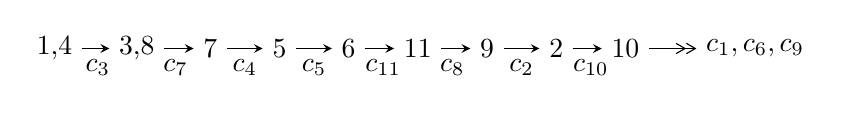
\begin{tikzpicture}[x=25pt, y=7pt]
	% node
	\node (A0) at (-1/8, 0) {1,4};
	\node (A1) at (17/16, 0) {3,8};
	\node (A2) at (17/8, 0) {7};
	\node (A3) at (25/8, 0) {5};
	\node (A4) at (33/8, 0) {6};
	\node (A5) at (41/8, 0) {11};
	\node (A6) at (49/8, 0) {9};
	\node (A7) at (57/8, 0) {2};
	\node (A8) at (65/8, 0) {10};
	\node (C1) at (1/2, -1) {$c_{3}$};
	\node (C2) at (13/8, -1) {$c_{7}$};
	\node (C3) at (21/8, -1) {$c_{4}$};
	\node (C4) at (29/8, -1) {$c_{5}$};
	\node (C5) at (37/8, -1) {$c_{11}$};
	\node (C6) at (45/8, -1) {$c_{8}$};
	\node (C7) at (53/8, -1) {$c_{2}$};
	\node (C8) at (61/8, -1) {$c_{10}$};
	\node (A9) at (10, 0) {$c_{1},c_{6},c_{9}$};

	% edge
	\draw[->,>=stealth]	
	(A0) edge (A1) (A1) edge (A2) (A2) edge (A3) (A3) edge (A4) (A4) edge (A5) (A5) edge (A6) (A6) edge (A7) (A7) edge (A8) ;
	\draw[->>,>={angle 60}]	
	(A8) edge (A9);
\end{tikzpicture} \\ 

\end{tabular} \\

\footnotetext{
The image of knot diagram is generated by the software ``\textbf{Draw programme}" developed by Andrew Bartholomew(\url{http://www.layer8.co.uk/maths/draw/index.htm\#Running-draw}), where we modified some parts for our purpose(\url{https://github.com/CATsTAILs/LinksPainter}).
}\phantom \\ \newline 
\centering \textbf{Ideals for irreducible components\footnotemark of $X_{\text{par}}$} 
 
\begin{align*}
I^u_{1}&=\langle 
-30442 u^{14}+342325 u^{13}+\cdots+44456 b+31712,\;-991 u^{14}+44316 u^{13}+\cdots+44456 a-908664,\\
\phantom{I^u_{1}}&\phantom{= \langle  }u^{15}-14 u^{14}+\cdots+464 u-32\rangle \\
I^u_{2}&=\langle 
-203 u^{17}-446 u^{16}+\cdots+16 b-99,\;-99 u^{17} a-1285 u^{17}+\cdots+606 a-2283,\\
\phantom{I^u_{2}}&\phantom{= \langle  }u^{18}+3 u^{17}+\cdots+9 u+1\rangle \\
I^u_{3}&=\langle 
-52 u^6-135 u^5-299 u^4-528 u^3-706 u^2+109 b-172 u-1,\\
\phantom{I^u_{3}}&\phantom{= \langle  }- u^6-55 u^5-142 u^4-312 u^3-546 u^2+109 a-716 u-174,\\
\phantom{I^u_{3}}&\phantom{= \langle  }u^7+3 u^6+7 u^5+13 u^4+18 u^3+10 u^2+2 u-1\rangle \\
I^u_{4}&=\langle 
a u+b+u-1,\;u^2 a+a^2-2 a u+u^2+2 a-3 u+3,\;u^3-2 u^2+u+1\rangle \\
\\
\end{align*}
\raggedright * 4 irreducible components of $\dim_{\mathbb{C}}=0$, with total 64 representations.\\
\footnotetext{All coefficients of polynomials are rational numbers. But the coefficients are sometimes approximated in decimal forms when there is not enough margin.}
\newpage
\renewcommand{\arraystretch}{1}
\centering \section*{I. $I^u_{1}= \langle -3.04\times10^{4} u^{14}+3.42\times10^{5} u^{13}+\cdots+4.45\times10^{4} b+3.17\times10^{4},\;-991 u^{14}+44316 u^{13}+\cdots+44456 a-908664,\;u^{15}-14 u^{14}+\cdots+464 u-32 \rangle$}
\flushleft \textbf{(i) Arc colorings}\\
\begin{tabular}{m{7pt} m{180pt} m{7pt} m{180pt} }
\flushright $a_{1}=$&$\begin{pmatrix}0\\u\end{pmatrix}$ \\
\flushright $a_{4}=$&$\begin{pmatrix}1\\0\end{pmatrix}$ \\
\flushright $a_{3}=$&$\begin{pmatrix}1\\- u^2\end{pmatrix}$ \\
\flushright $a_{8}=$&$\begin{pmatrix}0.0222917 u^{14}-0.996851 u^{13}+\cdots-194.288 u+20.4396\\0.684767 u^{14}-7.70031 u^{13}+\cdots-10.0963 u-0.713335\end{pmatrix}$ \\
\flushright $a_{7}=$&$\begin{pmatrix}0.707059 u^{14}-8.69716 u^{13}+\cdots-204.384 u+19.7263\\0.684767 u^{14}-7.70031 u^{13}+\cdots-10.0963 u-0.713335\end{pmatrix}$ \\
\flushright $a_{5}=$&$\begin{pmatrix}-0.120299 u^{14}+1.65732 u^{13}+\cdots+85.8621 u-8.43756\\-0.516758 u^{14}+6.69100 u^{13}+\cdots+180.708 u-12.6867\end{pmatrix}$ \\
\flushright $a_{6}=$&$\begin{pmatrix}-0.120299 u^{14}+1.65732 u^{13}+\cdots+85.8621 u-8.43756\\-0.692325 u^{14}+8.57538 u^{13}+\cdots+172.095 u-11.8272\end{pmatrix}$ \\
\flushright $a_{11}=$&$\begin{pmatrix}-0.396459 u^{14}+5.03367 u^{13}+\cdots+94.8459 u-3.24915\\0.516758 u^{14}-6.69100 u^{13}+\cdots-179.708 u+12.6867\end{pmatrix}$ \\
\flushright $a_{9}=$&$\begin{pmatrix}-2.35699 u^{14}+29.2392 u^{13}+\cdots+550.379 u-31.2776\\1.87224 u^{14}-24.4648 u^{13}+\cdots-743.922 u+53.5112\end{pmatrix}$ \\
\flushright $a_{2}=$&$\begin{pmatrix}0.442392 u^{14}-5.28185 u^{13}+\cdots-76.6178 u+5.65350\\-0.736076 u^{14}+9.23090 u^{13}+\cdots+209.229 u-15.0160\end{pmatrix}$ \\
\flushright $a_{10}=$&$\begin{pmatrix}-2.04145 u^{14}+25.4828 u^{13}+\cdots+540.956 u-35.1522\\1.84779 u^{14}-23.4858 u^{13}+\cdots-593.170 u+42.6315\end{pmatrix}$\\ \flushright $a_{10}=$&$\begin{pmatrix}-2.04145 u^{14}+25.4828 u^{13}+\cdots+540.956 u-35.1522\\1.84779 u^{14}-23.4858 u^{13}+\cdots-593.170 u+42.6315\end{pmatrix}$\\&\end{tabular}
\flushleft \textbf{(ii) Obstruction class $= -1$}\\~\\
\flushleft \textbf{(iii) Cusp Shapes $= -\frac{6047}{11114} u^{14}+\frac{56269}{11114} u^{13}+\cdots-\frac{448754}{5557} u-\frac{32342}{5557}$}\\~\\
\newpage\renewcommand{\arraystretch}{1}
\flushleft \textbf{(iv) u-Polynomials at the component}\newline \\
\begin{tabular}{m{50pt}|m{274pt}}
Crossings & \hspace{64pt}u-Polynomials at each crossing \\
\hline $$\begin{aligned}c_{1},c_{2},c_{5}\\c_{10}\end{aligned}$$&$\begin{aligned}
&u^{15}-5 u^{13}+\cdots+3 u+1
\end{aligned}$\\
\hline $$\begin{aligned}c_{3}\end{aligned}$$&$\begin{aligned}
&u^{15}-14 u^{14}+\cdots+464 u-32
\end{aligned}$\\
\hline $$\begin{aligned}c_{4},c_{7},c_{8}\\c_{11}\end{aligned}$$&$\begin{aligned}
&u^{15}- u^{14}+\cdots+4 u^2+1
\end{aligned}$\\
\hline $$\begin{aligned}c_{6},c_{9}\end{aligned}$$&$\begin{aligned}
&u^{15}-8 u^{14}+\cdots-56 u+8
\end{aligned}$\\
\hline
\end{tabular}\\~\\
\newpage\renewcommand{\arraystretch}{1}
\flushleft \textbf{(v) Riley Polynomials at the component}\newline \\
\begin{tabular}{m{50pt}|m{274pt}}
Crossings & \hspace{64pt}Riley Polynomials at each crossing \\
\hline $$\begin{aligned}c_{1},c_{2},c_{5}\\c_{10}\end{aligned}$$&$\begin{aligned}
&y^{15}-10 y^{14}+\cdots+29 y-1
\end{aligned}$\\
\hline $$\begin{aligned}c_{3}\end{aligned}$$&$\begin{aligned}
&y^{15}+4 y^{14}+\cdots+67328 y-1024
\end{aligned}$\\
\hline $$\begin{aligned}c_{4},c_{7},c_{8}\\c_{11}\end{aligned}$$&$\begin{aligned}
&y^{15}+7 y^{14}+\cdots-8 y-1
\end{aligned}$\\
\hline $$\begin{aligned}c_{6},c_{9}\end{aligned}$$&$\begin{aligned}
&y^{15}+8 y^{14}+\cdots+224 y-64
\end{aligned}$\\
\hline
\end{tabular}\\~\\
\newpage\flushleft \textbf{(vi) Complex Volumes and Cusp Shapes}
$$\begin{array}{c|c|c}  
\text{Solutions to }I^u_{1}& \I (\text{vol} + \sqrt{-1}CS) & \text{Cusp shape}\\
 \hline 
\begin{aligned}
u &= \phantom{-}0.441017 + 0.682615 I \\
a &= -0.626506 - 0.383690 I \\
b &= \phantom{-}0.014387 + 0.596876 I\end{aligned}
 & \phantom{-}1.16432 + 1.11480 I & \phantom{-}3.42758 - 4.27035 I \\ \hline\begin{aligned}
u &= \phantom{-}0.441017 - 0.682615 I \\
a &= -0.626506 + 0.383690 I \\
b &= \phantom{-}0.014387 - 0.596876 I\end{aligned}
 & \phantom{-}1.16432 - 1.11480 I & \phantom{-}3.42758 + 4.27035 I \\ \hline\begin{aligned}
u &= \phantom{-}1.360540 + 0.261249 I \\
a &= -0.645886 - 0.354688 I \\
b &= \phantom{-}0.786092 + 0.651305 I\end{aligned}
 & \phantom{-}1.20190 + 2.43151 I & -0.902369 - 0.814710 I \\ \hline\begin{aligned}
u &= \phantom{-}1.360540 - 0.261249 I \\
a &= -0.645886 + 0.354688 I \\
b &= \phantom{-}0.786092 - 0.651305 I\end{aligned}
 & \phantom{-}1.20190 - 2.43151 I & -0.902369 + 0.814710 I \\ \hline\begin{aligned}
u &= \phantom{-}0.231740 + 1.386460 I \\
a &= -0.727304 + 0.321329 I \\
b &= \phantom{-}0.614054 + 0.933909 I\end{aligned}
 & \phantom{-}7.18561 - 1.74581 I & \phantom{-}4.31703 + 3.15532 I \\ \hline\begin{aligned}
u &= \phantom{-}0.231740 - 1.386460 I \\
a &= -0.727304 - 0.321329 I \\
b &= \phantom{-}0.614054 - 0.933909 I\end{aligned}
 & \phantom{-}7.18561 + 1.74581 I & \phantom{-}4.31703 - 3.15532 I \\ \hline\begin{aligned}
u &= \phantom{-}1.38613 + 0.32674 I \\
a &= \phantom{-}0.553085 + 0.614738 I \\
b &= -0.565792 - 1.032820 I\end{aligned}
 & \phantom{-}0.37742 - 3.22470 I & \phantom{-}1.69059 + 1.81692 I \\ \hline\begin{aligned}
u &= \phantom{-}1.38613 - 0.32674 I \\
a &= \phantom{-}0.553085 - 0.614738 I \\
b &= -0.565792 + 1.032820 I\end{aligned}
 & \phantom{-}0.37742 + 3.22470 I & \phantom{-}1.69059 - 1.81692 I \\ \hline\begin{aligned}
u &= \phantom{-}1.03444 + 1.15733 I \\
a &= \phantom{-}0.878543 + 0.103476 I \\
b &= -0.789042 - 1.123810 I\end{aligned}
 & \phantom{-}0.98276 - 7.96105 I & \phantom{-}1.19655 + 6.90467 I \\ \hline\begin{aligned}
u &= \phantom{-}1.03444 - 1.15733 I \\
a &= \phantom{-}0.878543 - 0.103476 I \\
b &= -0.789042 + 1.123810 I\end{aligned}
 & \phantom{-}0.98276 + 7.96105 I & \phantom{-}1.19655 - 6.90467 I\\
 \hline 
 \end{array}$$\newpage$$\begin{array}{c|c|c}  
\text{Solutions to }I^u_{1}& \I (\text{vol} + \sqrt{-1}CS) & \text{Cusp shape}\\
 \hline 
\begin{aligned}
u &= \phantom{-}0.122764\phantom{ +0.000000I} \\
a &= \phantom{-}5.00969\phantom{ +0.000000I} \\
b &= -0.615011\phantom{ +0.000000I}\end{aligned}
 & -1.24987\phantom{ +0.000000I} & -10.6530\phantom{ +0.000000I} \\ \hline\begin{aligned}
u &= \phantom{-}1.41089 + 1.28897 I \\
a &= -0.730743 - 0.221034 I \\
b &= \phantom{-}0.74609 + 1.25376 I\end{aligned}
 & \phantom{-}4.8601 - 14.7989 I & \phantom{-}2.41187 + 8.28326 I \\ \hline\begin{aligned}
u &= \phantom{-}1.41089 - 1.28897 I \\
a &= -0.730743 + 0.221034 I \\
b &= \phantom{-}0.74609 - 1.25376 I\end{aligned}
 & \phantom{-}4.8601 + 14.7989 I & \phantom{-}2.41187 - 8.28326 I \\ \hline\begin{aligned}
u &= \phantom{-}1.07386 + 2.16285 I \\
a &= \phantom{-}0.293966 + 0.146746 I \\
b &= \phantom{-}0.001713 - 0.793388 I\end{aligned}
 & \phantom{-}6.23698 + 3.49716 I & \phantom{-}6.18530 - 1.96585 I \\ \hline\begin{aligned}
u &= \phantom{-}1.07386 - 2.16285 I \\
a &= \phantom{-}0.293966 - 0.146746 I \\
b &= \phantom{-}0.001713 + 0.793388 I\end{aligned}
 & \phantom{-}6.23698 - 3.49716 I & \phantom{-}6.18530 + 1.96585 I\\
 \hline 
 \end{array}$$\newpage\newpage\renewcommand{\arraystretch}{1}
\centering \section*{II. $I^u_{2}= \langle -203 u^{17}-446 u^{16}+\cdots+16 b-99,\;-99 u^{17} a-1285 u^{17}+\cdots+606 a-2283,\;u^{18}+3 u^{17}+\cdots+9 u+1 \rangle$}
\flushleft \textbf{(i) Arc colorings}\\
\begin{tabular}{m{7pt} m{180pt} m{7pt} m{180pt} }
\flushright $a_{1}=$&$\begin{pmatrix}0\\u\end{pmatrix}$ \\
\flushright $a_{4}=$&$\begin{pmatrix}1\\0\end{pmatrix}$ \\
\flushright $a_{3}=$&$\begin{pmatrix}1\\- u^2\end{pmatrix}$ \\
\flushright $a_{8}=$&$\begin{pmatrix}a\\12.6875 u^{17}+27.8750 u^{16}+\cdots+93.5625 u+6.18750\end{pmatrix}$ \\
\flushright $a_{7}=$&$\begin{pmatrix}\frac{203}{16} u^{17}+\frac{223}{8} u^{16}+\cdots+a+\frac{99}{16}\\12.6875 u^{17}+27.8750 u^{16}+\cdots+93.5625 u+6.18750\end{pmatrix}$ \\
\flushright $a_{5}=$&$\begin{pmatrix}-10.1875 a u^{17}-49.5625 u^{17}+\cdots-12.6875 a-109.375\\-10.1875 a u^{17}-10.8125 u^{17}+\cdots-12.6875 a-30.0625\end{pmatrix}$ \\
\flushright $a_{6}=$&$\begin{pmatrix}-10.1875 a u^{17}-49.5625 u^{17}+\cdots-12.6875 a-109.375\\-6 u^{17} a- u^{17}+\cdots-\frac{95}{16} a-8\end{pmatrix}$ \\
\flushright $a_{11}=$&$\begin{pmatrix}-12.6875 a u^{17}-38.7500 u^{17}+\cdots-6.18750 a-80.3125\\17.6875 u^{17}+45.1875 u^{16}+\cdots+269.438 u+38.7500\end{pmatrix}$ \\
\flushright $a_{9}=$&$\begin{pmatrix}-10.8125 a u^{17}+102.938 u^{17}+\cdots-29.0625 a+256.750\\-7.87500 a u^{17}+12.6875 u^{17}+\cdots-17.6875 a+6.18750\end{pmatrix}$ \\
\flushright $a_{2}=$&$\begin{pmatrix}-29.6875 a u^{17}-4.12500 u^{17}+\cdots-64.6250 a+32.9375\\-7 u^{17} a-\frac{109}{8} u^{17}+\cdots-\frac{119}{8} a-\frac{611}{16}\end{pmatrix}$ \\
\flushright $a_{10}=$&$\begin{pmatrix}-8.43750 a u^{17}+100.625 u^{17}+\cdots-10.3750 a+254.688\\-3.50000 a u^{17}+10.3750 u^{17}+\cdots-15.6875 a+4.12500\end{pmatrix}$\\ \flushright $a_{10}=$&$\begin{pmatrix}-8.43750 a u^{17}+100.625 u^{17}+\cdots-10.3750 a+254.688\\-3.50000 a u^{17}+10.3750 u^{17}+\cdots-15.6875 a+4.12500\end{pmatrix}$\\&\end{tabular}
\flushleft \textbf{(ii) Obstruction class $= -1$}\\~\\
\flushleft \textbf{(iii) Cusp Shapes $= \frac{371}{4} u^{17}+247 u^{16}+\frac{41}{4} u^{15}-\frac{3345}{4} u^{14}-\frac{4809}{4} u^{13}-1271 u^{12}+\frac{1677}{4} u^{11}+\frac{23513}{4} u^{10}+6462 u^9-\frac{13723}{2} u^8-\frac{21065}{2} u^7+\frac{13659}{2} u^6+\frac{38345}{4} u^5-\frac{6133}{2} u^4-\frac{13047}{4} u^3+\frac{7575}{4} u^2+1672 u+\frac{585}{2}$}\\~\\
\newpage\renewcommand{\arraystretch}{1}
\flushleft \textbf{(iv) u-Polynomials at the component}\newline \\
\begin{tabular}{m{50pt}|m{274pt}}
Crossings & \hspace{64pt}u-Polynomials at each crossing \\
\hline $$\begin{aligned}c_{1},c_{2},c_{5}\\c_{10}\end{aligned}$$&$\begin{aligned}
&u^{36}-10 u^{34}+\cdots+503 u+161
\end{aligned}$\\
\hline $$\begin{aligned}c_{3}\end{aligned}$$&$\begin{aligned}
&(u^{18}+3 u^{17}+\cdots+9 u+1)^{2}
\end{aligned}$\\
\hline $$\begin{aligned}c_{4},c_{7},c_{8}\\c_{11}\end{aligned}$$&$\begin{aligned}
&u^{36}-2 u^{35}+\cdots-151 u+47
\end{aligned}$\\
\hline $$\begin{aligned}c_{6},c_{9}\end{aligned}$$&$\begin{aligned}
&(u^{18}+3 u^{17}+\cdots+4 u+5)^{2}
\end{aligned}$\\
\hline
\end{tabular}\\~\\
\newpage\renewcommand{\arraystretch}{1}
\flushleft \textbf{(v) Riley Polynomials at the component}\newline \\
\begin{tabular}{m{50pt}|m{274pt}}
Crossings & \hspace{64pt}Riley Polynomials at each crossing \\
\hline $$\begin{aligned}c_{1},c_{2},c_{5}\\c_{10}\end{aligned}$$&$\begin{aligned}
&y^{36}-20 y^{35}+\cdots-295835 y+25921
\end{aligned}$\\
\hline $$\begin{aligned}c_{3}\end{aligned}$$&$\begin{aligned}
&(y^{18}-7 y^{17}+\cdots-31 y+1)^{2}
\end{aligned}$\\
\hline $$\begin{aligned}c_{4},c_{7},c_{8}\\c_{11}\end{aligned}$$&$\begin{aligned}
&y^{36}+16 y^{35}+\cdots+18277 y+2209
\end{aligned}$\\
\hline $$\begin{aligned}c_{6},c_{9}\end{aligned}$$&$\begin{aligned}
&(y^{18}+11 y^{17}+\cdots+174 y+25)^{2}
\end{aligned}$\\
\hline
\end{tabular}\\~\\
\newpage\flushleft \textbf{(vi) Complex Volumes and Cusp Shapes}
$$\begin{array}{c|c|c}  
\text{Solutions to }I^u_{2}& \I (\text{vol} + \sqrt{-1}CS) & \text{Cusp shape}\\
 \hline 
\begin{aligned}
u &= \phantom{-}0.894501 + 0.439989 I \\
a &= -1.068970 - 0.589062 I \\
b &= \phantom{-}1.172180 - 0.401841 I\end{aligned}
 & \phantom{-}2.21070 - 8.01702 I & \phantom{-}0.26506 + 6.04046 I \\ \hline\begin{aligned}
u &= \phantom{-}0.894501 + 0.439989 I \\
a &= -0.877218 + 0.880723 I \\
b &= \phantom{-}0.697017 + 0.997253 I\end{aligned}
 & \phantom{-}2.21070 - 8.01702 I & \phantom{-}0.26506 + 6.04046 I \\ \hline\begin{aligned}
u &= \phantom{-}0.894501 - 0.439989 I \\
a &= -1.068970 + 0.589062 I \\
b &= \phantom{-}1.172180 + 0.401841 I\end{aligned}
 & \phantom{-}2.21070 + 8.01702 I & \phantom{-}0.26506 - 6.04046 I \\ \hline\begin{aligned}
u &= \phantom{-}0.894501 - 0.439989 I \\
a &= -0.877218 - 0.880723 I \\
b &= \phantom{-}0.697017 - 0.997253 I\end{aligned}
 & \phantom{-}2.21070 + 8.01702 I & \phantom{-}0.26506 - 6.04046 I \\ \hline\begin{aligned}
u &= -0.950537 + 0.162221 I \\
a &= -0.971317 + 0.562568 I \\
b &= \phantom{-}0.732831 + 0.297516 I\end{aligned}
 & -1.79766 + 2.11512 I & -3.46832 - 4.22083 I \\ \hline\begin{aligned}
u &= -0.950537 + 0.162221 I \\
a &= \phantom{-}0.697241 + 0.431990 I \\
b &= -0.832013 + 0.692310 I\end{aligned}
 & -1.79766 + 2.11512 I & -3.46832 - 4.22083 I \\ \hline\begin{aligned}
u &= -0.950537 - 0.162221 I \\
a &= -0.971317 - 0.562568 I \\
b &= \phantom{-}0.732831 - 0.297516 I\end{aligned}
 & -1.79766 - 2.11512 I & -3.46832 + 4.22083 I \\ \hline\begin{aligned}
u &= -0.950537 - 0.162221 I \\
a &= \phantom{-}0.697241 - 0.431990 I \\
b &= -0.832013 - 0.692310 I\end{aligned}
 & -1.79766 - 2.11512 I & -3.46832 + 4.22083 I \\ \hline\begin{aligned}
u &= \phantom{-}0.550574 + 0.534542 I \\
a &= \phantom{-}1.151550 + 0.184083 I \\
b &= -1.137440 + 0.607496 I\end{aligned}
 & -0.695457 - 1.211150 I & \phantom{-}2.01684 + 5.97065 I \\ \hline\begin{aligned}
u &= \phantom{-}0.550574 + 0.534542 I \\
a &= \phantom{-}0.51202 - 1.60050 I \\
b &= -0.535612 - 0.716902 I\end{aligned}
 & -0.695457 - 1.211150 I & \phantom{-}2.01684 + 5.97065 I\\
 \hline 
 \end{array}$$\newpage$$\begin{array}{c|c|c}  
\text{Solutions to }I^u_{2}& \I (\text{vol} + \sqrt{-1}CS) & \text{Cusp shape}\\
 \hline 
\begin{aligned}
u &= \phantom{-}0.550574 - 0.534542 I \\
a &= \phantom{-}1.151550 - 0.184083 I \\
b &= -1.137440 - 0.607496 I\end{aligned}
 & -0.695457 + 1.211150 I & \phantom{-}2.01684 - 5.97065 I \\ \hline\begin{aligned}
u &= \phantom{-}0.550574 - 0.534542 I \\
a &= \phantom{-}0.51202 + 1.60050 I \\
b &= -0.535612 + 0.716902 I\end{aligned}
 & -0.695457 + 1.211150 I & \phantom{-}2.01684 - 5.97065 I \\ \hline\begin{aligned}
u &= -0.559442 + 0.038809 I \\
a &= -1.60100 + 1.20636 I \\
b &= \phantom{-}0.620068 + 1.024030 I\end{aligned}
 & \phantom{-}0.388234 - 1.127970 I & \phantom{-}1.85464 + 1.58148 I \\ \hline\begin{aligned}
u &= -0.559442 + 0.038809 I \\
a &= \phantom{-}0.97669 + 1.89819 I \\
b &= -0.848848 + 0.737023 I\end{aligned}
 & \phantom{-}0.388234 - 1.127970 I & \phantom{-}1.85464 + 1.58148 I \\ \hline\begin{aligned}
u &= -0.559442 - 0.038809 I \\
a &= -1.60100 - 1.20636 I \\
b &= \phantom{-}0.620068 - 1.024030 I\end{aligned}
 & \phantom{-}0.388234 + 1.127970 I & \phantom{-}1.85464 - 1.58148 I \\ \hline\begin{aligned}
u &= -0.559442 - 0.038809 I \\
a &= \phantom{-}0.97669 - 1.89819 I \\
b &= -0.848848 - 0.737023 I\end{aligned}
 & \phantom{-}0.388234 + 1.127970 I & \phantom{-}1.85464 - 1.58148 I \\ \hline\begin{aligned}
u &= -1.20149 + 0.95062 I \\
a &= -0.794303 + 0.267048 I \\
b &= \phantom{-}0.590660 - 0.737715 I\end{aligned}
 & -0.58133 + 3.63224 I & -1.22357 - 0.72654 I \\ \hline\begin{aligned}
u &= -1.20149 + 0.95062 I \\
a &= \phantom{-}0.601110 - 0.138403 I \\
b &= -0.700489 + 1.075930 I\end{aligned}
 & -0.58133 + 3.63224 I & -1.22357 - 0.72654 I \\ \hline\begin{aligned}
u &= -1.20149 - 0.95062 I \\
a &= -0.794303 - 0.267048 I \\
b &= \phantom{-}0.590660 + 0.737715 I\end{aligned}
 & -0.58133 - 3.63224 I & -1.22357 + 0.72654 I \\ \hline\begin{aligned}
u &= -1.20149 - 0.95062 I \\
a &= \phantom{-}0.601110 + 0.138403 I \\
b &= -0.700489 - 1.075930 I\end{aligned}
 & -0.58133 - 3.63224 I & -1.22357 + 0.72654 I\\
 \hline 
 \end{array}$$\newpage$$\begin{array}{c|c|c}  
\text{Solutions to }I^u_{2}& \I (\text{vol} + \sqrt{-1}CS) & \text{Cusp shape}\\
 \hline 
\begin{aligned}
u &= \phantom{-}1.57847 + 0.07406 I \\
a &= -0.056442 - 0.945021 I \\
b &= \phantom{-}0.253884 + 0.746014 I\end{aligned}
 & \phantom{-}8.78344 + 0.53962 I & \phantom{-}4.04425 + 2.43806 I \\ \hline\begin{aligned}
u &= \phantom{-}1.57847 + 0.07406 I \\
a &= -0.182614 - 0.464051 I \\
b &= \phantom{-}0.01910 + 1.49587 I\end{aligned}
 & \phantom{-}8.78344 + 0.53962 I & \phantom{-}4.04425 + 2.43806 I \\ \hline\begin{aligned}
u &= \phantom{-}1.57847 - 0.07406 I \\
a &= -0.056442 + 0.945021 I \\
b &= \phantom{-}0.253884 - 0.746014 I\end{aligned}
 & \phantom{-}8.78344 - 0.53962 I & \phantom{-}4.04425 - 2.43806 I \\ \hline\begin{aligned}
u &= \phantom{-}1.57847 - 0.07406 I \\
a &= -0.182614 + 0.464051 I \\
b &= \phantom{-}0.01910 - 1.49587 I\end{aligned}
 & \phantom{-}8.78344 - 0.53962 I & \phantom{-}4.04425 - 2.43806 I \\ \hline\begin{aligned}
u &= -0.305821 + 0.029607 I \\
a &= \phantom{-}0.52691 + 2.98749 I \\
b &= \phantom{-}0.20657 - 1.64071 I\end{aligned}
 & \phantom{-}9.40827 - 2.73362 I & \phantom{-}5.19032 + 6.28765 I \\ \hline\begin{aligned}
u &= -0.305821 + 0.029607 I \\
a &= \phantom{-}1.18377 - 5.25035 I \\
b &= \phantom{-}0.249590 + 0.898036 I\end{aligned}
 & \phantom{-}9.40827 - 2.73362 I & \phantom{-}5.19032 + 6.28765 I \\ \hline\begin{aligned}
u &= -0.305821 - 0.029607 I \\
a &= \phantom{-}0.52691 - 2.98749 I \\
b &= \phantom{-}0.20657 + 1.64071 I\end{aligned}
 & \phantom{-}9.40827 + 2.73362 I & \phantom{-}5.19032 - 6.28765 I \\ \hline\begin{aligned}
u &= -0.305821 - 0.029607 I \\
a &= \phantom{-}1.18377 + 5.25035 I \\
b &= \phantom{-}0.249590 - 0.898036 I\end{aligned}
 & \phantom{-}9.40827 + 2.73362 I & \phantom{-}5.19032 - 6.28765 I \\ \hline\begin{aligned}
u &= \phantom{-}0.08820 + 1.71388 I \\
a &= \phantom{-}0.440400 + 0.416925 I \\
b &= \phantom{-}0.047819 + 0.888995 I\end{aligned}
 & \phantom{-}6.66136 + 3.28569 I & \phantom{-}5.54170 - 2.88739 I \\ \hline\begin{aligned}
u &= \phantom{-}0.08820 + 1.71388 I \\
a &= -0.518764 + 0.001204 I \\
b &= \phantom{-}0.675718 - 0.791567 I\end{aligned}
 & \phantom{-}6.66136 + 3.28569 I & \phantom{-}5.54170 - 2.88739 I\\
 \hline 
 \end{array}$$\newpage$$\begin{array}{c|c|c}  
\text{Solutions to }I^u_{2}& \I (\text{vol} + \sqrt{-1}CS) & \text{Cusp shape}\\
 \hline 
\begin{aligned}
u &= \phantom{-}0.08820 - 1.71388 I \\
a &= \phantom{-}0.440400 - 0.416925 I \\
b &= \phantom{-}0.047819 - 0.888995 I\end{aligned}
 & \phantom{-}6.66136 - 3.28569 I & \phantom{-}5.54170 + 2.88739 I \\ \hline\begin{aligned}
u &= \phantom{-}0.08820 - 1.71388 I \\
a &= -0.518764 - 0.001204 I \\
b &= \phantom{-}0.675718 + 0.791567 I\end{aligned}
 & \phantom{-}6.66136 - 3.28569 I & \phantom{-}5.54170 + 2.88739 I \\ \hline\begin{aligned}
u &= -1.59445 + 1.02172 I \\
a &= \phantom{-}0.595268 - 0.396932 I \\
b &= -0.754617 + 0.978635 I\end{aligned}
 & \phantom{-}1.11892 + 7.08645 I & \phantom{-}2.27907 - 7.07165 I \\ \hline\begin{aligned}
u &= -1.59445 + 1.02172 I \\
a &= -0.614327 + 0.220117 I \\
b &= \phantom{-}0.543574 - 1.241090 I\end{aligned}
 & \phantom{-}1.11892 + 7.08645 I & \phantom{-}2.27907 - 7.07165 I \\ \hline\begin{aligned}
u &= -1.59445 - 1.02172 I \\
a &= \phantom{-}0.595268 + 0.396932 I \\
b &= -0.754617 - 0.978635 I\end{aligned}
 & \phantom{-}1.11892 - 7.08645 I & \phantom{-}2.27907 + 7.07165 I \\ \hline\begin{aligned}
u &= -1.59445 - 1.02172 I \\
a &= -0.614327 - 0.220117 I \\
b &= \phantom{-}0.543574 + 1.241090 I\end{aligned}
 & \phantom{-}1.11892 - 7.08645 I & \phantom{-}2.27907 + 7.07165 I\\
 \hline 
 \end{array}$$\newpage\newpage\renewcommand{\arraystretch}{1}
\centering \section*{III. $I^u_{3}= \langle -52 u^6-135 u^5+\cdots+109 b-1,\;- u^6-55 u^5+\cdots+109 a-174,\;u^7+3 u^6+7 u^5+13 u^4+18 u^3+10 u^2+2 u-1 \rangle$}
\flushleft \textbf{(i) Arc colorings}\\
\begin{tabular}{m{7pt} m{180pt} m{7pt} m{180pt} }
\flushright $a_{1}=$&$\begin{pmatrix}0\\u\end{pmatrix}$ \\
\flushright $a_{4}=$&$\begin{pmatrix}1\\0\end{pmatrix}$ \\
\flushright $a_{3}=$&$\begin{pmatrix}1\\- u^2\end{pmatrix}$ \\
\flushright $a_{8}=$&$\begin{pmatrix}0.00917431 u^{6}+0.504587 u^{5}+\cdots+6.56881 u+1.59633\\0.477064 u^{6}+1.23853 u^{5}+\cdots+1.57798 u+0.00917431\end{pmatrix}$ \\
\flushright $a_{7}=$&$\begin{pmatrix}0.486239 u^{6}+1.74312 u^{5}+\cdots+8.14679 u+1.60550\\0.477064 u^{6}+1.23853 u^{5}+\cdots+1.57798 u+0.00917431\end{pmatrix}$ \\
\flushright $a_{5}=$&$\begin{pmatrix}-0.339450 u^{6}-0.669725 u^{5}+\cdots+2.95413 u+2.93578\\0.100917 u^{6}+0.550459 u^{5}+\cdots+3.25688 u-0.440367\end{pmatrix}$ \\
\flushright $a_{6}=$&$\begin{pmatrix}-0.339450 u^{6}-0.669725 u^{5}+\cdots+2.95413 u+2.93578\\-0.0275229 u^{6}+0.486239 u^{5}+\cdots+4.29358 u-0.788991\end{pmatrix}$ \\
\flushright $a_{11}=$&$\begin{pmatrix}-0.440367 u^{6}-1.22018 u^{5}+\cdots-0.302752 u+2.37615\\0.100917 u^{6}+0.550459 u^{5}+\cdots+4.25688 u-0.440367\end{pmatrix}$ \\
\flushright $a_{9}=$&$\begin{pmatrix}0.899083 u^{6}+2.44954 u^{5}+\cdots+6.74312 u+2.44037\\-0.440367 u^{6}-1.22018 u^{5}+\cdots-0.302752 u+1.37615\end{pmatrix}$ \\
\flushright $a_{2}=$&$\begin{pmatrix}1.33945 u^{6}+3.66972 u^{5}+\cdots+7.04587 u+0.0642202\\-0.220183 u^{6}-1.11009 u^{5}+\cdots-4.65138 u+1.68807\end{pmatrix}$ \\
\flushright $a_{10}=$&$\begin{pmatrix}0.889908 u^{6}+1.94495 u^{5}+\cdots+0.174312 u-0.155963\\-0.788991 u^{6}-2.39450 u^{5}+\cdots-3.91743 u+1.71560\end{pmatrix}$\\ \flushright $a_{10}=$&$\begin{pmatrix}0.889908 u^{6}+1.94495 u^{5}+\cdots+0.174312 u-0.155963\\-0.788991 u^{6}-2.39450 u^{5}+\cdots-3.91743 u+1.71560\end{pmatrix}$\\&\end{tabular}
\flushleft \textbf{(ii) Obstruction class $= 1$}\\~\\
\flushleft \textbf{(iii) Cusp Shapes $= -\frac{56}{109} u^6-\frac{246}{109} u^5-\frac{431}{109} u^4-\frac{904}{109} u^3-\frac{1146}{109} u^2-\frac{856}{109} u+\frac{611}{109}$}\\~\\
\newpage\renewcommand{\arraystretch}{1}
\flushleft \textbf{(iv) u-Polynomials at the component}\newline \\
\begin{tabular}{m{50pt}|m{274pt}}
Crossings & \hspace{64pt}u-Polynomials at each crossing \\
\hline $$\begin{aligned}c_{1},c_{10}\end{aligned}$$&$\begin{aligned}
&u^7-2 u^5-2 u^4+u^3+2 u^2+2 u+1
\end{aligned}$\\
\hline $$\begin{aligned}c_{2},c_{5}\end{aligned}$$&$\begin{aligned}
&u^7-2 u^5+2 u^4+u^3-2 u^2+2 u-1
\end{aligned}$\\
\hline $$\begin{aligned}c_{3}\end{aligned}$$&$\begin{aligned}
&u^7+3 u^6+7 u^5+13 u^4+18 u^3+10 u^2+2 u-1
\end{aligned}$\\
\hline $$\begin{aligned}c_{4},c_{8}\end{aligned}$$&$\begin{aligned}
&u^7- u^6+3 u^5-2 u^4+3 u^3- u^2+u-1
\end{aligned}$\\
\hline $$\begin{aligned}c_{6}\end{aligned}$$&$\begin{aligned}
&u^7- u^6+3 u^5-2 u^4+u^3- u^2- u-1
\end{aligned}$\\
\hline $$\begin{aligned}c_{7},c_{11}\end{aligned}$$&$\begin{aligned}
&u^7+u^6+3 u^5+2 u^4+3 u^3+u^2+u+1
\end{aligned}$\\
\hline $$\begin{aligned}c_{9}\end{aligned}$$&$\begin{aligned}
&u^7+u^6+3 u^5+2 u^4+u^3+u^2- u+1
\end{aligned}$\\
\hline
\end{tabular}\\~\\
\newpage\renewcommand{\arraystretch}{1}
\flushleft \textbf{(v) Riley Polynomials at the component}\newline \\
\begin{tabular}{m{50pt}|m{274pt}}
Crossings & \hspace{64pt}Riley Polynomials at each crossing \\
\hline $$\begin{aligned}c_{1},c_{2},c_{5}\\c_{10}\end{aligned}$$&$\begin{aligned}
&y^7-4 y^6+6 y^5-4 y^4+y^3+4 y^2-1
\end{aligned}$\\
\hline $$\begin{aligned}c_{3}\end{aligned}$$&$\begin{aligned}
&y^7+5 y^6+7 y^5+27 y^4+98 y^3-2 y^2+24 y-1
\end{aligned}$\\
\hline $$\begin{aligned}c_{4},c_{7},c_{8}\\c_{11}\end{aligned}$$&$\begin{aligned}
&y^7+5 y^6+11 y^5+14 y^4+9 y^3+y^2- y-1
\end{aligned}$\\
\hline $$\begin{aligned}c_{6},c_{9}\end{aligned}$$&$\begin{aligned}
&y^7+5 y^6+7 y^5-2 y^4-11 y^3-7 y^2- y-1
\end{aligned}$\\
\hline
\end{tabular}\\~\\
\newpage\flushleft \textbf{(vi) Complex Volumes and Cusp Shapes}
$$\begin{array}{c|c|c}  
\text{Solutions to }I^u_{3}& \I (\text{vol} + \sqrt{-1}CS) & \text{Cusp shape}\\
 \hline 
\begin{aligned}
u &= -0.508137 + 0.486029 I \\
a &= -1.22583 + 1.38607 I \\
b &= -0.050784 - 1.300110 I\end{aligned}
 & \phantom{-}11.34660 + 1.05141 I & \phantom{-}8.13453 - 0.52743 I \\ \hline\begin{aligned}
u &= -0.508137 - 0.486029 I \\
a &= -1.22583 - 1.38607 I \\
b &= -0.050784 + 1.300110 I\end{aligned}
 & \phantom{-}11.34660 - 1.05141 I & \phantom{-}8.13453 + 0.52743 I \\ \hline\begin{aligned}
u &= -1.35766 + 0.93784 I \\
a &= -0.676700 + 0.313046 I \\
b &= \phantom{-}0.625140 - 1.059640 I\end{aligned}
 & -0.00156 + 5.16496 I & \phantom{-}0.90846 - 5.47109 I \\ \hline\begin{aligned}
u &= -1.35766 - 0.93784 I \\
a &= -0.676700 - 0.313046 I \\
b &= \phantom{-}0.625140 + 1.059640 I\end{aligned}
 & -0.00156 - 5.16496 I & \phantom{-}0.90846 + 5.47109 I \\ \hline\begin{aligned}
u &= \phantom{-}0.203752\phantom{ +0.000000I} \\
a &= \phantom{-}3.16933\phantom{ +0.000000I} \\
b &= \phantom{-}0.645755\phantom{ +0.000000I}\end{aligned}
 & -0.607992\phantom{ +0.000000I} & \phantom{-}3.49110\phantom{ +0.000000I} \\ \hline\begin{aligned}
u &= \phantom{-}0.26392 + 1.89105 I \\
a &= \phantom{-}0.317866 + 0.254422 I \\
b &= -0.397234 + 0.668248 I\end{aligned}
 & \phantom{-}5.40832 + 4.21557 I & -0.78856 - 7.31442 I \\ \hline\begin{aligned}
u &= \phantom{-}0.26392 - 1.89105 I \\
a &= \phantom{-}0.317866 - 0.254422 I \\
b &= -0.397234 - 0.668248 I\end{aligned}
 & \phantom{-}5.40832 - 4.21557 I & -0.78856 + 7.31442 I\\
 \hline 
 \end{array}$$\newpage\newpage\renewcommand{\arraystretch}{1}
\centering \section*{IV. $I^u_{4}= \langle a u+b+u-1,\;u^2 a+a^2-2 a u+u^2+2 a-3 u+3,\;u^3-2 u^2+u+1 \rangle$}
\flushleft \textbf{(i) Arc colorings}\\
\begin{tabular}{m{7pt} m{180pt} m{7pt} m{180pt} }
\flushright $a_{1}=$&$\begin{pmatrix}0\\u\end{pmatrix}$ \\
\flushright $a_{4}=$&$\begin{pmatrix}1\\0\end{pmatrix}$ \\
\flushright $a_{3}=$&$\begin{pmatrix}1\\- u^2\end{pmatrix}$ \\
\flushright $a_{8}=$&$\begin{pmatrix}a\\- a u- u+1\end{pmatrix}$ \\
\flushright $a_{7}=$&$\begin{pmatrix}- a u+a- u+1\\- a u- u+1\end{pmatrix}$ \\
\flushright $a_{5}=$&$\begin{pmatrix}u^2 a- a u\\u^2 a- a u+u^2-2 u\end{pmatrix}$ \\
\flushright $a_{6}=$&$\begin{pmatrix}u^2 a- a u\\a u+u^2+a-2 u\end{pmatrix}$ \\
\flushright $a_{11}=$&$\begin{pmatrix}- a u+u^2+a-2 u+1\\u+1\end{pmatrix}$ \\
\flushright $a_{9}=$&$\begin{pmatrix}u^2 a-2 a u+u^2+a-2 u+2\\u^2 a- u+1\end{pmatrix}$ \\
\flushright $a_{2}=$&$\begin{pmatrix}u^2 a- a u+1\\-2 u^2 a+3 a u- u^2+2 a+u+1\end{pmatrix}$ \\
\flushright $a_{10}=$&$\begin{pmatrix}u^2 a-2 a u+u^2-2 u+1\\2 u^2 a- a u- a- u\end{pmatrix}$\\ \flushright $a_{10}=$&$\begin{pmatrix}u^2 a-2 a u+u^2-2 u+1\\2 u^2 a- a u- a- u\end{pmatrix}$\\&\end{tabular}
\flushleft \textbf{(ii) Obstruction class $= 1$}\\~\\
\flushleft \textbf{(iii) Cusp Shapes $= -4 u^2+6 u+1$}\\~\\
\newpage\renewcommand{\arraystretch}{1}
\flushleft \textbf{(iv) u-Polynomials at the component}\newline \\
\begin{tabular}{m{50pt}|m{274pt}}
Crossings & \hspace{64pt}u-Polynomials at each crossing \\
\hline $$\begin{aligned}c_{1},c_{10}\end{aligned}$$&$\begin{aligned}
&u^6+3 u^5+u^4-3 u^3- u^2+u+1
\end{aligned}$\\
\hline $$\begin{aligned}c_{2},c_{5}\end{aligned}$$&$\begin{aligned}
&u^6-3 u^5+u^4+3 u^3- u^2- u+1
\end{aligned}$\\
\hline $$\begin{aligned}c_{3}\end{aligned}$$&$\begin{aligned}
&(u^3-2 u^2+u+1)^2
\end{aligned}$\\
\hline $$\begin{aligned}c_{4},c_{8}\end{aligned}$$&$\begin{aligned}
&u^6- u^5+3 u^4-3 u^3+3 u^2- u+1
\end{aligned}$\\
\hline $$\begin{aligned}c_{6}\end{aligned}$$&$\begin{aligned}
&(u^3+u-1)^2
\end{aligned}$\\
\hline $$\begin{aligned}c_{7},c_{11}\end{aligned}$$&$\begin{aligned}
&u^6+u^5+3 u^4+3 u^3+3 u^2+u+1
\end{aligned}$\\
\hline $$\begin{aligned}c_{9}\end{aligned}$$&$\begin{aligned}
&(u^3+u+1)^2
\end{aligned}$\\
\hline
\end{tabular}\\~\\
\newpage\renewcommand{\arraystretch}{1}
\flushleft \textbf{(v) Riley Polynomials at the component}\newline \\
\begin{tabular}{m{50pt}|m{274pt}}
Crossings & \hspace{64pt}Riley Polynomials at each crossing \\
\hline $$\begin{aligned}c_{1},c_{2},c_{5}\\c_{10}\end{aligned}$$&$\begin{aligned}
&y^6-7 y^5+17 y^4-15 y^3+9 y^2-3 y+1
\end{aligned}$\\
\hline $$\begin{aligned}c_{3}\end{aligned}$$&$\begin{aligned}
&(y^3-2 y^2+5 y-1)^2
\end{aligned}$\\
\hline $$\begin{aligned}c_{4},c_{7},c_{8}\\c_{11}\end{aligned}$$&$\begin{aligned}
&y^6+5 y^5+9 y^4+9 y^3+9 y^2+5 y+1
\end{aligned}$\\
\hline $$\begin{aligned}c_{6},c_{9}\end{aligned}$$&$\begin{aligned}
&(y^3+2 y^2+y-1)^2
\end{aligned}$\\
\hline
\end{tabular}\\~\\
\newpage\flushleft \textbf{(vi) Complex Volumes and Cusp Shapes}
$$\begin{array}{c|c|c}  
\text{Solutions to }I^u_{4}& \I (\text{vol} + \sqrt{-1}CS) & \text{Cusp shape}\\
 \hline 
\begin{aligned}
u &= \phantom{-}1.23279 + 0.79255 I \\
a &= -0.632657 - 0.782837 I \\
b &= -0.073295 + 0.673932 I\end{aligned}
 & \phantom{-}8.79110 + 1.58317 I & \phantom{-}4.83023 - 3.06106 I \\ \hline\begin{aligned}
u &= \phantom{-}1.23279 + 0.79255 I \\
a &= \phantom{-}0.206606 + 0.413848 I \\
b &= -0.15949 - 1.46648 I\end{aligned}
 & \phantom{-}8.79110 + 1.58317 I & \phantom{-}4.83023 - 3.06106 I \\ \hline\begin{aligned}
u &= \phantom{-}1.23279 - 0.79255 I \\
a &= -0.632657 + 0.782837 I \\
b &= -0.073295 - 0.673932 I\end{aligned}
 & \phantom{-}8.79110 - 1.58317 I & \phantom{-}4.83023 + 3.06106 I \\ \hline\begin{aligned}
u &= \phantom{-}1.23279 - 0.79255 I \\
a &= \phantom{-}0.206606 - 0.413848 I \\
b &= -0.15949 + 1.46648 I\end{aligned}
 & \phantom{-}8.79110 - 1.58317 I & \phantom{-}4.83023 + 3.06106 I \\ \hline\begin{aligned}
u &= -0.465571\phantom{ +0.000000I} \\
a &= -1.57395 + 1.46156 I \\
b &= \phantom{-}0.732786 + 0.680460 I\end{aligned}
 & -1.13287\phantom{ +0.000000I} & -2.66050\phantom{ +0.000000I} \\ \hline\begin{aligned}
u &= -0.465571\phantom{ +0.000000I} \\
a &= -1.57395 - 1.46156 I \\
b &= \phantom{-}0.732786 - 0.680460 I\end{aligned}
 & -1.13287\phantom{ +0.000000I} & -2.66050\phantom{ +0.000000I}\\
 \hline 
 \end{array}$$\newpage
\newpage\renewcommand{\arraystretch}{1}
\centering \section*{ V. u-Polynomials}
\begin{tabular}{m{50pt}|m{274pt}}
Crossings & \hspace{64pt}u-Polynomials at each crossing \\
\hline $$\begin{aligned}c_{1},c_{10}\end{aligned}$$&$\begin{aligned}
&(u^6+3 u^5+u^4-3 u^3- u^2+u+1)(u^7-2 u^5-2 u^4+u^3+2 u^2+2 u+1)\\
&\cdot(u^{15}-5 u^{13}+\cdots+3 u+1)(u^{36}-10 u^{34}+\cdots+503 u+161)
\end{aligned}$\\
\hline $$\begin{aligned}c_{2},c_{5}\end{aligned}$$&$\begin{aligned}
&(u^6-3 u^5+u^4+3 u^3- u^2- u+1)(u^7-2 u^5+2 u^4+u^3-2 u^2+2 u-1)\\
&\cdot(u^{15}-5 u^{13}+\cdots+3 u+1)(u^{36}-10 u^{34}+\cdots+503 u+161)
\end{aligned}$\\
\hline $$\begin{aligned}c_{3}\end{aligned}$$&$\begin{aligned}
&(u^3-2 u^2+u+1)^2(u^7+3 u^6+7 u^5+13 u^4+18 u^3+10 u^2+2 u-1)\\
&\cdot(u^{15}-14 u^{14}+\cdots+464 u-32)(u^{18}+3 u^{17}+\cdots+9 u+1)^{2}
\end{aligned}$\\
\hline $$\begin{aligned}c_{4},c_{8}\end{aligned}$$&$\begin{aligned}
&(u^6- u^5+3 u^4-3 u^3+3 u^2- u+1)\\
&\cdot(u^7- u^6+\cdots+u-1)(u^{15}- u^{14}+\cdots+4 u^2+1)\\
&\cdot(u^{36}-2 u^{35}+\cdots-151 u+47)
\end{aligned}$\\
\hline $$\begin{aligned}c_{6}\end{aligned}$$&$\begin{aligned}
&(u^3+u-1)^2(u^7- u^6+3 u^5-2 u^4+u^3- u^2- u-1)\\
&\cdot(u^{15}-8 u^{14}+\cdots-56 u+8)(u^{18}+3 u^{17}+\cdots+4 u+5)^{2}
\end{aligned}$\\
\hline $$\begin{aligned}c_{7},c_{11}\end{aligned}$$&$\begin{aligned}
&(u^6+u^5+3 u^4+3 u^3+3 u^2+u+1)\\
&\cdot(u^7+u^6+\cdots+u+1)(u^{15}- u^{14}+\cdots+4 u^2+1)\\
&\cdot(u^{36}-2 u^{35}+\cdots-151 u+47)
\end{aligned}$\\
\hline $$\begin{aligned}c_{9}\end{aligned}$$&$\begin{aligned}
&(u^3+u+1)^2(u^7+u^6+3 u^5+2 u^4+u^3+u^2- u+1)\\
&\cdot(u^{15}-8 u^{14}+\cdots-56 u+8)(u^{18}+3 u^{17}+\cdots+4 u+5)^{2}
\end{aligned}$\\
\hline
\end{tabular}\newpage\renewcommand{\arraystretch}{1}
\centering \section*{ VI. Riley Polynomials}
\begin{tabular}{m{50pt}|m{274pt}}
Crossings & \hspace{64pt}Riley Polynomials at each crossing \\
\hline $$\begin{aligned}c_{1},c_{2},c_{5}\\c_{10}\end{aligned}$$&$\begin{aligned}
&(y^6-7 y^5+17 y^4-15 y^3+9 y^2-3 y+1)\\
&\cdot(y^7-4 y^6+\cdots+4 y^2-1)(y^{15}-10 y^{14}+\cdots+29 y-1)\\
&\cdot(y^{36}-20 y^{35}+\cdots-295835 y+25921)
\end{aligned}$\\
\hline $$\begin{aligned}c_{3}\end{aligned}$$&$\begin{aligned}
&((y^3-2 y^2+5 y-1)^2)(y^7+5 y^6+\cdots+24 y-1)\\
&\cdot(y^{15}+4 y^{14}+\cdots+67328 y-1024)(y^{18}-7 y^{17}+\cdots-31 y+1)^{2}
\end{aligned}$\\
\hline $$\begin{aligned}c_{4},c_{7},c_{8}\\c_{11}\end{aligned}$$&$\begin{aligned}
&(y^6+5 y^5+9 y^4+9 y^3+9 y^2+5 y+1)\\
&\cdot(y^7+5 y^6+\cdots- y-1)(y^{15}+7 y^{14}+\cdots-8 y-1)\\
&\cdot(y^{36}+16 y^{35}+\cdots+18277 y+2209)
\end{aligned}$\\
\hline $$\begin{aligned}c_{6},c_{9}\end{aligned}$$&$\begin{aligned}
&(y^3+2 y^2+y-1)^2(y^7+5 y^6+7 y^5-2 y^4-11 y^3-7 y^2- y-1)\\
&\cdot(y^{15}+8 y^{14}+\cdots+224 y-64)(y^{18}+11 y^{17}+\cdots+174 y+25)^{2}
\end{aligned}$\\
\hline
\end{tabular}
\vskip 2pc
\end{document}